%% 5章用 (Brent)

以下の図表は，Brent法による極値探索を用いて，関数 $f(x) = \frac{1}{1+25x^2}$ ($n=15$) を近似した際の収束過程を示したものである．

表\ref{tab:remes-brent-log}は，各反復で算出された参照均等誤差 $|E|$ と，Brent法で高精度に求められた実際の最大誤差，およびその差の推移である．
グリッド極値点探索と比較して，より高精度な収束（$10^{-15}$ オーダー）が達成されている．

図\ref{fig:remes-brent-convergence}は，反復に伴う誤差の収束過程を可視化したものである．
Brent法により，機械イプシロン精度に近い等振動性が実現されていることが確認できる．


\begin{figure}[H]
 \centering
 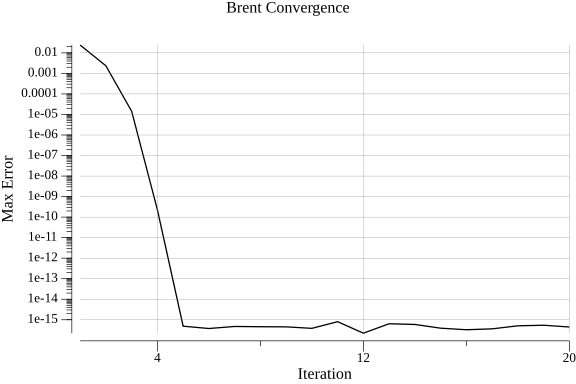
\includegraphics[width=0.6\linewidth]{material/remes/outputs/brent/convergence_brent.png}
 \caption{Brent法による最大誤差の収束履歴}
 \label{fig:remes-brent-convergence}
\end{figure}

\begin{figure}[H]
 \centering
 \begin{minipage}[b]{0.48\textwidth}
  \centering
  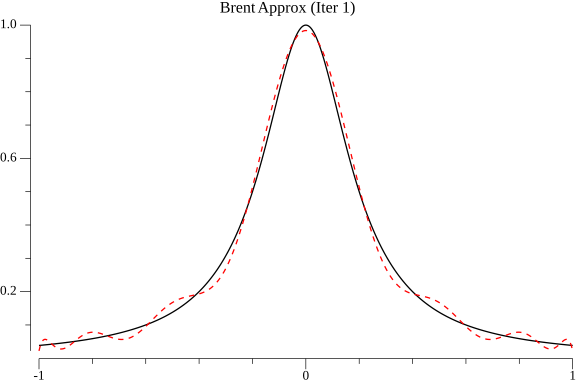
\includegraphics[width=1.0\linewidth]{material/remes/outputs/brent/func_remes_brent_iter01.png}
  \caption{Iter 1}
 \end{minipage}
 \hfill
 \begin{minipage}[b]{0.48\textwidth}
  \centering
  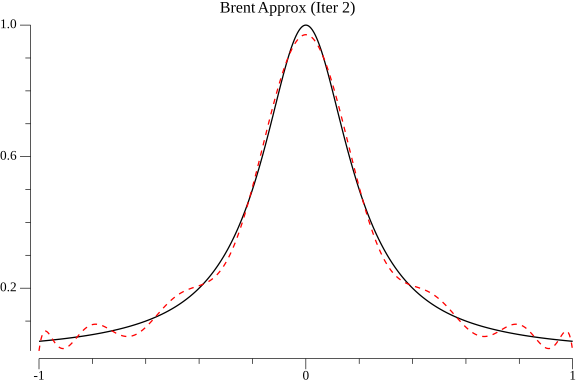
\includegraphics[width=1.0\linewidth]{material/remes/outputs/brent/func_remes_brent_iter02.png}
  \caption{Iter 2}
 \end{minipage}

 \begin{minipage}[b]{0.48\textwidth}
  \centering
  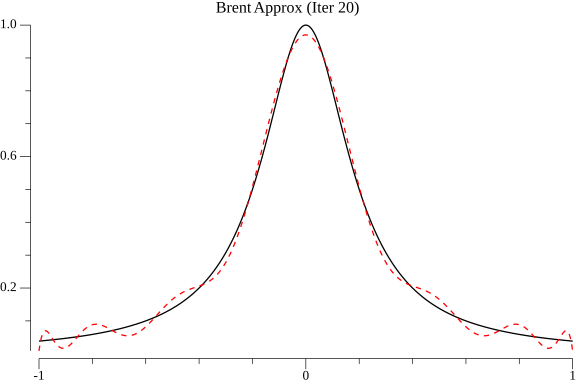
\includegraphics[width=1.0\linewidth]{material/remes/outputs/brent/func_remes_brent_iter20.png}
  \caption{Iter 20}
 \end{minipage}

 \caption{Brent法: 近似多項式の推移}
 \label{fig:remes-brent-approx}
\end{figure}
\begin{figure}[H]
 \centering
 \begin{minipage}[b]{0.48\textwidth}
  \centering
  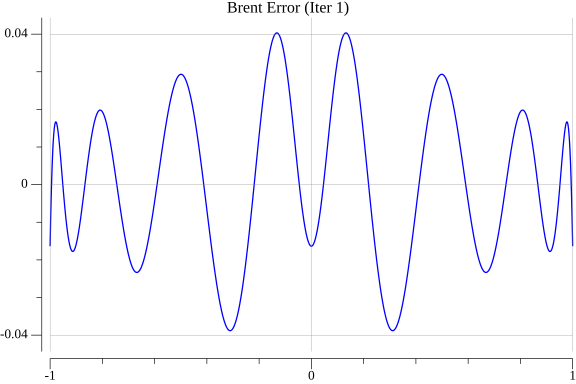
\includegraphics[width=1.0\linewidth]{material/remes/outputs/brent/error_remes_brent_iter01.png}
  \caption{Iter 1}
 \end{minipage}
 \hfill
 \begin{minipage}[b]{0.48\textwidth}
  \centering
  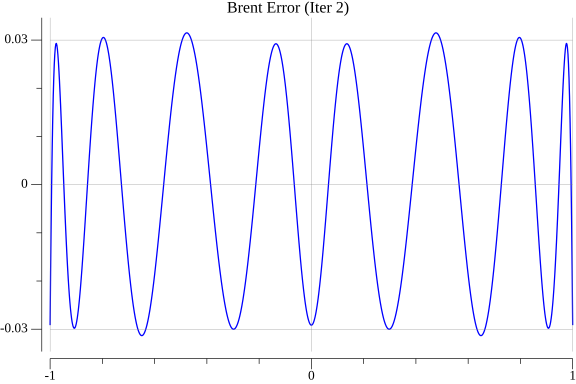
\includegraphics[width=1.0\linewidth]{material/remes/outputs/brent/error_remes_brent_iter02.png}
  \caption{Iter 2}
 \end{minipage}

 \begin{minipage}[b]{0.48\textwidth}
  \centering
  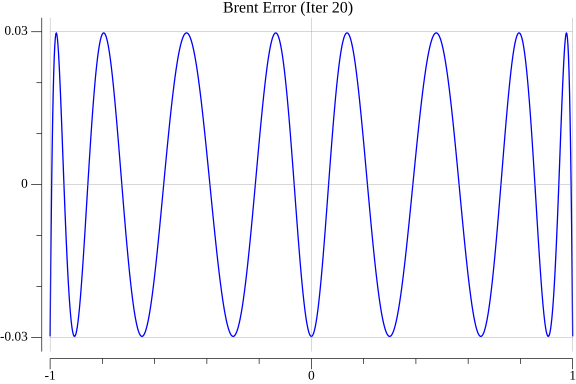
\includegraphics[width=1.0\linewidth]{material/remes/outputs/brent/error_remes_brent_iter20.png}
  \caption{Iter 20}
 \end{minipage}

 \caption{Brent法: 誤差関数の推移}
 \label{fig:remes-brent-error}
\end{figure}

\begin{table}[H]
 \centering
 \caption{Brent法の収束ログ}
 \label{tab:remes-brent-log}
 \begin{tabular}{crrrr}
 \toprule
 Iter & $|E|$ & Coeff Norm & Node Move & Error Change \\
 \midrule
 1 & $1.63552e-02$ & $0.00000e+00$ & $0.00000e+00$ & $0.00000e+00$ \\
 2 & $2.91586e-02$ & $1.38180e-02$ & $4.97122e-02$ & $1.28034e-02$ \\
 3 & $2.97711e-02$ & $1.27592e-03$ & $3.72393e-03$ & $6.12455e-04$ \\
 4 & $2.97767e-02$ & $6.60148e-06$ & $1.24099e-05$ & $5.62755e-06$ \\
 5 & $2.97767e-02$ & $1.05586e-10$ & $5.25736e-09$ & $9.91564e-11$ \\
 6 & $2.97767e-02$ & $1.62634e-16$ & $5.64624e-09$ & $6.24500e-17$ \\
 7 & $2.97767e-02$ & $2.07658e-16$ & $4.94056e-09$ & $6.93889e-18$ \\
 8 & $2.97767e-02$ & $2.55847e-16$ & $4.96228e-09$ & $2.42861e-17$ \\
 9 & $2.97767e-02$ & $1.62274e-16$ & $3.21817e-09$ & $3.46945e-18$ \\
 10 & $2.97767e-02$ & $2.38584e-16$ & $3.65966e-09$ & $6.93889e-18$ \\
 11 & $2.97767e-02$ & $2.28951e-16$ & $4.44502e-09$ & $1.73472e-17$ \\
 12 & $2.97767e-02$ & $2.19203e-16$ & $3.89086e-09$ & $0.00000e+00$ \\
 13 & $2.97767e-02$ & $1.66362e-16$ & $4.61242e-09$ & $6.93889e-18$ \\
 14 & $2.97767e-02$ & $2.27033e-16$ & $4.29365e-09$ & $2.42861e-17$ \\
 15 & $2.97767e-02$ & $2.48827e-16$ & $4.68158e-09$ & $2.77556e-17$ \\
 16 & $2.97767e-02$ & $1.87220e-16$ & $5.47251e-09$ & $5.89806e-17$ \\
 17 & $2.97767e-02$ & $1.19187e-16$ & $6.30429e-09$ & $7.97973e-17$ \\
 18 & $2.97767e-02$ & $1.93991e-16$ & $3.62033e-09$ & $3.12250e-17$ \\
 19 & $2.97767e-02$ & $2.77619e-16$ & $4.55541e-09$ & $7.63278e-17$ \\
 20 & $2.97767e-02$ & $1.85424e-16$ & $5.41280e-09$ & $7.63278e-17$ \\
 \bottomrule
 \end{tabular}
\end{table}

\begin{table}[H]
 \centering
 \caption{Brent法利用時の誤差の再評価}
 \label{tab:remes-brent-final-check}
 \begin{tabular}{crrr}
 \toprule
 No. & 収束時誤差 & 再評価誤差 & 差分 \\
 \midrule
 1 & $2.97766890e-02$ & $2.97766890e-02$ & $9.60343e-15$ \\
 2 & $2.97766890e-02$ & $2.97766890e-02$ & $0.00000e+00$ \\
 3 & $2.97766890e-02$ & $2.97766890e-02$ & $-1.38778e-17$ \\
 4 & $2.97766890e-02$ & $2.97766890e-02$ & $6.93889e-18$ \\
 5 & $2.97766890e-02$ & $2.97766890e-02$ & $0.00000e+00$ \\
 6 & $2.97766890e-02$ & $2.97766890e-02$ & $-2.77556e-17$ \\
 7 & $2.97766890e-02$ & $2.97766890e-02$ & $0.00000e+00$ \\
 8 & $2.97766890e-02$ & $2.97766890e-02$ & $0.00000e+00$ \\
 9 & $2.97766890e-02$ & $2.97766890e-02$ & $0.00000e+00$ \\
 10 & $2.97766890e-02$ & $2.97766890e-02$ & $0.00000e+00$ \\
 11 & $2.97766890e-02$ & $2.97766890e-02$ & $0.00000e+00$ \\
 12 & $2.97766890e-02$ & $2.97766890e-02$ & $-2.77556e-17$ \\
 13 & $2.97766890e-02$ & $2.97766890e-02$ & $-6.93889e-18$ \\
 14 & $2.97766890e-02$ & $2.97766890e-02$ & $-1.38778e-17$ \\
 15 & $2.97766890e-02$ & $2.97766890e-02$ & $6.93889e-18$ \\
 16 & $2.97766890e-02$ & $2.97766890e-02$ & $0.00000e+00$ \\
 17 & $2.97766890e-02$ & $2.97766890e-02$ & $8.93036e-15$ \\
 \bottomrule
 \end{tabular}
\vspace{1mm}

\small \textbf{注：}
\small 上表は，区間 $[-1.0,1.0]$ を探索するRemesアルゴリズムによって導かれた誤差関数に対する表である．

\small 収束時誤差とはBrent法をもちいることで極値点探索を行ったRemesアルゴリズムで導出された誤差関数の各極値点で観測された誤差である．

\small 再評価誤差とはBrent法という極値点探索アルゴリズムにより観測された誤差の絶対値である．

\[
 \text{観測された最大誤差} \; \|E\|_{\max}^{\text{strict}}(f) = \max_{x \in [-1.0,1.0]} |f(x) - p^*(x)| \approx 2.97766890e-02 .
 \]
\end{table}
